\newpage

\section{Задание 7.}

Найти поток векторного поля $\vv{a}(x, y, z)$ через замкнутую поверхность S (нормаль внешняя). Вычислить двумя способами: с помощью поверхностного и тройного интеграла.

$$\vv{a} = y\vv{i} + 5y\vv{j} + z\vv{k}, \quad S: x^2 + y^2 = 1, \quad z = x, \quad z = 0, \quad z \geq 0$$

\begin{figure}[h!t]
    \centering
    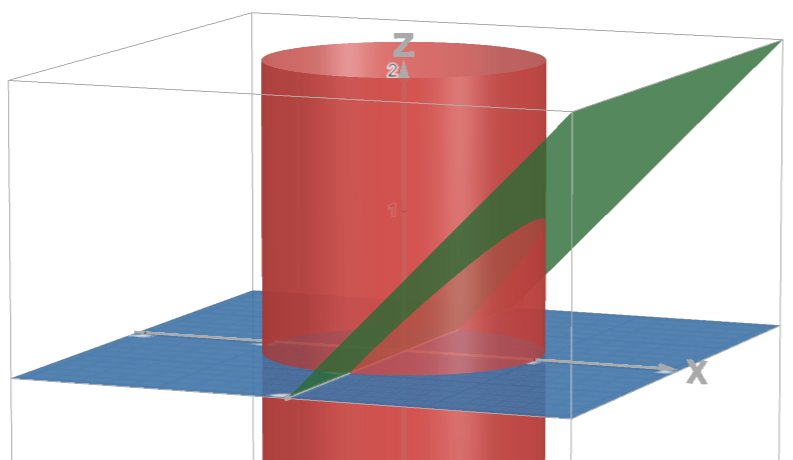
\includegraphics[width=0.5\linewidth]{Task7/Surfaces_closing_the_figure.png}
    \caption{Задание 7. Поверхности, задающие фигуру.\underline{\href{https://www.desmos.com/3d/pfnmmjbtkb}{(Desmos)}}.}
\end{figure}

\subsection{Решение с помощью тройного интеграла.}

Воспользуемся теоремой Остроградского-Гаусса.

$$\Pi_S(\vv{a}) = \iint \limits_S \vv{a} \cdot \vv{N_0} \, dS = \iiint \limits_V (\text{div}\vv{a})\,dV$$

Посчитаем дивергенцию векторного поля $\vv{a}$.
$$\text{div}\vv{a} = \nabla \cdot \vv{a} = \dfrac{\partial}{\partial x}\left(y\right) + \dfrac{\partial}{\partial y}\left(5y\right) + \dfrac{\partial}{\partial z}\left(z\right) = 0 + 5 + 1 = 6$$

Теперь подставим.

$$\iiint \limits_V (\text{div}\vv{a})\,dV = 6 \iiint \limits_V \,dV$$

Перейдем в цилиндрические координаты. Причем, для нашей фигуры нужно ограничить переменные следующим образом. 
$$
\begin{cases}
    x=r\cos{\phi}\\
    y=r\sin{\phi}\\
    z=z
\end{cases} ; \quad
\begin{cases}
    z\geq0\\
    z=x
\end{cases} \Rightarrow \quad
\begin{cases}
    z\geq0\\
    z = r\cos{\phi}
\end{cases} \Rightarrow \quad
\begin{cases}
    \cos{\phi} \geq 0 \\
    \phi \in [-\pi/2, \pi/2]
\end{cases} \Rightarrow \quad
\begin{cases}
    r \in [0,1]\\
    \phi \in [-\pi/2, \pi/2]\\
    z\in[0, r\cos{\phi}]
\end{cases}$$

Теперь мы можем сделать замену, учитывая $\left| J\right| = r$ 

$$6 \iiint \limits_V \,dV = 6 \int_0^1\,dr \int_{-\pi/2}^{\pi/2} \,d\phi \int_0^{r\cos{\phi}} r\, dz = 6 \int_0^1\,dr \int_{-\pi/2}^{\pi/2} r^2\cos{\phi}\,d\phi = 6 \int_0^1 r^2 \left[-\sin{\phi}\right]_{-\pi/2}^{\pi/2} \,dr =$$ 
$$= 6 \int_0^1 r^2 \cdot 2 \,dr = 12 \cdot \dfrac{1}{3} = \boxed{4}.$$


\subsection{Решение с помощью поверхностного интеграла.}

$$\Pi_S(\vv{a}) = \iint \limits_S \vv{a} \cdot \vv{N_0} d\vv{S}$$

По свойству аддитивности интеграла, разобьем его на три: нижняя крышка, кусок цилиндра и верхняя крышка. 

$$\iint \limits_S = \iint \limits_{\text{нижняя крышка}} + \iint \limits_{\text{верхняя крышка}} + \iint \limits_{\text{кусок цилиндра}}$$
\begin{center}

Теперь найдем векторы нормали для каждого интеграла.
\begin{figure}[h!t]
    \centering
    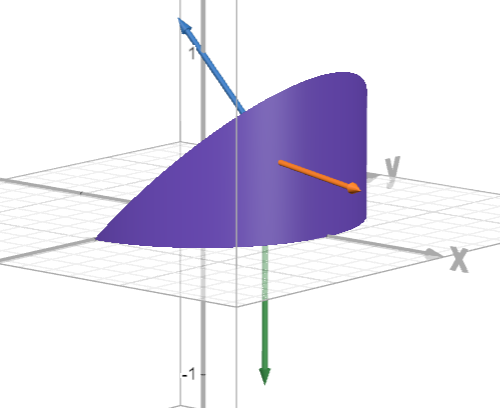
\includegraphics[width=0.5\linewidth]{Task7/Normal_vectors_of_the_figure.png}
    \caption{Задание 7. Векторы нормали фигуры. \underline{\href{https://www.desmos.com/3d/aebkcx5iql}{(Desmos)}}.}
\end{figure}

    Для нижней крышки (зеленая стрелка) $\vv{N_0} = (0,0,-1)$\\
    Для верхней крышки (синяя стрелка) $\vv{N_0} = (-\sqrt{2}/2, 0,\sqrt{2}/2)$\\
    Для куска цилиндра (оранжевая стрелка) $\vv{N_0}(\phi) = (\cos{\phi}, \sin{\phi}, 0)$

Теперь можно рассмотреть каждый интеграл по отдельности.

$$\iint \limits_{\text{нижняя крышка}} \vv{a} \cdot \vv{N_0} d\vv{S} = 
\iint \limits_{\text{нижняя крышка}} (y,5y,z) \cdot (0,0,-1) d\vv{S} = 
\iint \limits_{\text{нижняя крышка}} -z\, d\vv{S} = 0$$

Так как нижняя крышка задается уравнением $z=0$, то этот интеграл будет равен нулю.

$$\iint \limits_{\text{верхняя крышка}} \vv{a} \cdot \vv{N_0} d\vv{S} = \iint \limits_{\text{верхняя крышка}} (y,5y,z) \cdot (-\sqrt{2}/2, 0,\sqrt{2}/2) d\vv{S} = \dfrac{\sqrt{2}}{2} \iint \limits_{\text{верхняя крышка}} (-y + z) d\vv{S}$$

Мы можем выразить $z$ через $x$, т.к. эта поверхность задается уравнением $z=x$. Теперь $z(x,y) = x$.

$$d\vv{S} = \sqrt{1 + \left(\frac{\partial z}{\partial x}\right)^2 + \left(\frac{\partial z}{\partial y}\right)^2} \,dx\,dy = \sqrt{1 + \left(\frac{\partial x}{\partial x}\right)^2 + \left(\frac{\partial x}{\partial y}\right)^2} \,dx\,dy = \sqrt{2}\,dx\,dy$$

$$\dfrac{\sqrt{2}}{2} \iint \limits_{\text{верхняя крышка}} (-y + z) d\vv{S} = \sqrt{2} \cdot \dfrac{\sqrt{2}}{2} \iint \limits_{x^2 + y^2\leq1 \{x\geq0\}} (-y + x) \,dx\,dy$$
Перейдем в полярные координаты.
$$\iint \limits_{x^2 + y^2\leq1 \{x\geq0\}} (-y + x) \,dx\,dy = \int_{-\pi/2}^{\pi/2} d\phi \int_0^1 (-r\sin{\phi} + r\cos{\phi}) \cdot r \, dr = \dfrac{1}{3}\int_{-\pi/2}^{\pi/2} \cos{\phi} - \sin{\phi}\,d\phi = $$

$$= \dfrac{1}{3} \left[\sin{\phi}+\cos{\phi}\right]_{-\pi/2}^{\pi/2} = \dfrac{1}{3} \left[1+0-(-1+0)\right] = \dfrac{2}{3}$$

Теперь последний интеграл.
Сразу перейдем в цилиндрические координаты, чтобы можно было пользоваться вектором нормали. Тут $r=const=1$, тогда $|J| = 1$.

$$
\begin{cases}
    x=\cos{\phi}\\
    y=\sin{\phi}\\
    z=z
\end{cases}
$$
Так как эта поверхность ограничена сверху плоскостью $z=x$, можно выразить $z$ через $x$.

$$
\begin{cases}
    x=\cos{\phi}\\
    z=x
\end{cases}\Rightarrow \quad z\in[0, \cos{\phi}]
$$
$$\iint \limits_{\text{кусок цилиндра}} \vv{a} \cdot \vv{N_0} d\vv{S} = 
\int_{-\pi/2}^{\pi/2}\, d\phi \int_{0}^{\cos{\phi}} \left((\sin{\phi}, 5\sin{\phi}, z) \cdot (\cos{\phi}, \sin{\phi}, 0)\right)\,dz = $$
$$=\int_{-\pi/2}^{\pi/2}\, \left(\sin{\phi}\cos{\phi} +  5\sin^2{\phi}\right)\cos{\phi}\, d\phi = \int_{-\pi/2}^{\pi/2}\, \sin{\phi}\cos^2{\phi} + 5\sin^2{\phi}\cos{\phi}\, d\phi = $$ 
$$= \int_{-\pi/2}^{\pi/2} \sin{\phi}\cos^2{\phi}\, d\phi + \int_{-\pi/2}^{\pi/2} 5\sin^2{\phi}\cos{\phi}\, d\phi$$

Рассмотрим левый интеграл и сразу сделаем замену переменной пусть $u=\cos{\phi}$, $du = -\sin{\phi}\,d\phi$
$$\int_{-\pi/2}^{\pi/2} \sin{\phi}\cos^2{\phi}\, d\phi = -\int_{0}^{0} u^2\, du = 0$$

Рассмотрим правый интеграл и сразу сделаем замену переменной пусть $u=\sin{\phi}$, $du = \cos{\phi}\,d\phi$

$$\int_{-\pi/2}^{\pi/2} 5\sin^2{\phi}\cos{\phi}\, d\phi = \int_{-1}^{1} 5u^2 \, du = 5 \cdot \left[\dfrac{u^3}{3}\right]_{-1}^1 = 5 \cdot \left[\dfrac{1}{3} - \left(-\dfrac{1}{3}\right)\right] = \dfrac{10}{3}$$

Теперь сложим полученные значения трех интегралов.

$$0 + \dfrac{2}{3} + \dfrac{10}{3} = \dfrac{12}{3} = \boxed{4}$$

Ответы сошлись, значит всё правильно :)

\end{center}
